% !TEX program = xelatex
% Question 4: The Plot-Twist Generator -- build from this folder with: tectonic report.tex   (or: latexmk -xelatex report.tex)
% Same layout as Question-2/report/report.tex. Figures are read from ../outputs/figures/.
\documentclass[10pt,a4paper]{article}

\usepackage[margin=1.9cm]{geometry}
\usepackage{fontspec}            % XeLaTeX / tectonic: Latin Modern, plus a Devanagari font for the Hindi examples
\usepackage{amsmath,amssymb}
\usepackage{graphicx}
\usepackage{booktabs}
\usepackage{longtable}
\usepackage{array}
\usepackage{calc}
\usepackage{etoolbox}
\usepackage{xcolor}
\usepackage{microtype}
\usepackage[font=small,labelfont=bf,skip=4pt]{caption}
\usepackage{enumitem}
\usepackage[colorlinks=true,linkcolor=black,citecolor=black,urlcolor=blue!50!black]{hyperref}

% Hindi: first Devanagari font that is installed (Noto is on Overleaf and in the fonts-noto-core package)
\IfFontExistsTF{Noto Serif Devanagari}{\newfontfamily\hindifont[Script=Devanagari]{Noto Serif Devanagari}}{%
\IfFontExistsTF{Noto Sans Devanagari}{\newfontfamily\hindifont[Script=Devanagari]{Noto Sans Devanagari}}{%
\IfFontExistsTF{FreeSerif}{\newfontfamily\hindifont[Script=Devanagari]{FreeSerif}}{%
\newfontfamily\hindifont[Script=Devanagari]{Latin Modern Roman}}}}
\DeclareRobustCommand{\hi}[1]{{\hindifont #1}}

\makeatletter
\def\maxwidth{\ifdim\Gin@nat@width>\linewidth\linewidth\else\Gin@nat@width\fi}
\def\maxheight{\ifdim\Gin@nat@height>0.34\textheight 0.34\textheight\else\Gin@nat@height\fi}
\makeatother
\setkeys{Gin}{width=\maxwidth,height=\maxheight,keepaspectratio}
\setlist{itemsep=1pt,topsep=2pt,parsep=0pt}
\setlength{\parskip}{3pt}
\setlength{\parindent}{0pt}
\setlength{\emergencystretch}{3em}
\renewcommand{\arraystretch}{1.12}
\renewcommand{\floatpagefraction}{0.85}
\setcounter{secnumdepth}{-\maxdimen}   % section numbers are typed into the headings
\AtBeginEnvironment{longtable}{\footnotesize}
\providecommand{\tightlist}{\setlength{\itemsep}{0pt}\setlength{\parskip}{0pt}}
\newcommand{\code}[1]{\texttt{#1}}

\title{\vspace{-1.2cm}\textbf{Question 4: The Plot-Twist Generator}\\[2pt]
\large DSL 504 Natural Language Processing, Group Assignment 2}
\author{Akshat Gupta}
\date{November 2026}

\begin{document}
\maketitle
\vspace{-0.6cm}

Vanilla RNN vs LSTM story language models on TinyStories, three decoding strategies, diversity metrics, and a blinded
human evaluation. Author: Akshat Gupta. All numbers below come from the files in \texttt{outputs/results/}; commands to
reproduce them are in \href{README.md}{\texttt{README.md}}.

\textbf{Human evaluation.} Four teammates (Ayush, Keshav, Rishi Kharya, Shivam Singh) rated the same 20 blinded stories; I did not
rate, so no author ratings are included. Their raw CSVs are in \texttt{outputs/human\_eval/ratings/}. The main result is that
the raters agree with each other very little (Section 6.3), and that no rating difference between the two models is
statistically distinguishable from zero with 10 matched pairs.

\hypertarget{summary}{%
\section{1. Summary}\label{summary}}

\begin{longtable}[]{@{}
  >{\raggedright\arraybackslash}p{(\columnwidth - 4\tabcolsep) * \real{0.3333}}
  >{\raggedright\arraybackslash}p{(\columnwidth - 4\tabcolsep) * \real{0.3333}}
  >{\raggedright\arraybackslash}p{(\columnwidth - 4\tabcolsep) * \real{0.3333}}@{}}
\toprule\noalign{}
\begin{minipage}[b]{\linewidth}\raggedright
\end{minipage} & \begin{minipage}[b]{\linewidth}\raggedright
Vanilla RNN
\end{minipage} & \begin{minipage}[b]{\linewidth}\raggedright
LSTM
\end{minipage} \\
\midrule\noalign{}
\endhead
\bottomrule\noalign{}
\endlastfoot
Parameters & 5,418,886 & 6,601,606 \\
Validation / test perplexity (seed 42) & 16.44 / 16.15 & \textbf{12.12 / 11.86} \\
Test perplexity, mean \ensuremath{\pm} std over 2 seeds & 16.14 \ensuremath{\pm} 0.02 & \textbf{11.79 \ensuremath{\pm} 0.09} \\
Training time, 25 epochs, GTX 1650 & 25.9 min & 39.7 min \\
Repetition rate, greedy & 0.444 & 0.420 \\
Repetition rate, temp 0.8 & 0.026 & 0.038 \\
Stories that never end within 250 tokens, temp 0.8 & 17.5\% & \textbf{8.4\%} \\
\end{longtable}

The LSTM has a clearly lower perplexity (about 27\% lower), more stories that finish properly, and keeps a character's
name more often. It does not clearly tell better stories: both models are
word-salad-prone, both loop under greedy decoding, and the RNN is the \emph{less} repetitive one at the same temperature.
Neither model produced a twist in any of the five Plot-Twist openings. In the blinded human ratings (4 raters, 20 stories) the LSTM
scored higher on coherence (+0.30) and relevance (+0.28), the RNN higher on grammar (+0.25) and creativity (+0.12), and the overall difference was +0.05
for the LSTM with a 95\% interval of {[}-0.22, +0.36{]}, i.e.~a tie. The lower perplexity did not buy a measurably better storyteller.

\hypertarget{data-and-preprocessing-part-1}{%
\section{2. Data and preprocessing (Part 1)}\label{data-and-preprocessing-part-1}}

\textbf{Subset.} \texttt{roneneldan/TinyStories} (the brief spells the id \texttt{roneldan}, which does not exist on the Hub).
20,000 training, 1,000 validation and 1,000 test stories, the sizes the brief suggests. The training set is a seeded
sample (seed 42) from the first 60,000 filtered stories of the official train split. Validation and test are disjoint
seeded samples of the official validation split. 23 held-out stories that were exact duplicates of a training story were
removed. Stories longer than 400 tokens were dropped rather than truncated (4,032 from the train pool, 1,170 from the
validation split), so every training sequence is a complete story with its real ending. No dataset files are part of
the submission; \texttt{data\_summary.json} stores a hash per split.

The split is made at the story level before any sequence is built, so no part of a story can leak between splits.

\begin{longtable}[]{@{}llll@{}}
\toprule\noalign{}
split & stories & tokens & median story length \\
\midrule\noalign{}
\endhead
\bottomrule\noalign{}
\endlastfoot
train & 20,000 & 3,728,248 & 174 \\
validation & 1,000 & 185,224 & 174 \\
test & 1,000 & 185,087 & 174 \\
\end{longtable}

\textbf{Tokenisation.} Lower-cased word-level tokens, punctuation as separate tokens, contractions kept whole.
1,242 training stories contained mojibake (broken UTF-8 quotes) and were repaired before tokenising. One vocabulary
is built from the training split only; words seen fewer than 5 times become \texttt{\textless{}unk\textgreater{}}. Vocabulary size is 6,534
(6,530 words plus \texttt{\textless{}pad\textgreater{}}, \texttt{\textless{}unk\textgreater{}}, \texttt{\textless{}sos\textgreater{}}, \texttt{\textless{}eos\textgreater{}}); it covers 99.75\% of training tokens. Both models use the same
tokens and the same vocabulary.

\textbf{Sequences and next-token pairs.} One story is one sequence: \texttt{\textless{}sos\textgreater{}\ w1\ ...\ wn\ \textless{}eos\textgreater{}}. The input is the sequence
without its last token and the target is the sequence without its first, so the model sees \texttt{w\_t} and must predict
\texttt{w\_\{t+1\}}. A worked example is in \texttt{outputs/results/next\_token\_example.md}:

\begin{longtable}[]{@{}lll@{}}
\toprule\noalign{}
step & input & target \\
\midrule\noalign{}
\endhead
\bottomrule\noalign{}
\endlastfoot
0 & \texttt{\textless{}sos\textgreater{}} & \texttt{once} \\
1 & \texttt{once} & \texttt{upon} \\
2 & \texttt{upon} & \texttt{a} \\
\ldots{} & \ldots{} & \ldots{} \\
181 & \texttt{.} & \texttt{\textless{}eos\textgreater{}} \\
\end{longtable}

\textbf{Why story boundaries are preserved.} A story is a closed narrative: characters, setting and the goal of the
plot all live inside it. If a window straddled two stories the model would be trained to predict the opening of
one story from the ending of an unrelated one, which teaches nonsense transitions. Keeping \texttt{\textless{}sos\textgreater{}} and \texttt{\textless{}eos\textgreater{}} at the
true boundaries also means the model learns what an opening and an ending look like, which it needs in order to stop
by itself at generation time. It also makes the split clean (no story, or fragment of one, in two splits).

\textbf{How padding is handled.} Stories have different lengths, so each batch is padded on the right with \texttt{\textless{}pad\textgreater{}}.
The loss uses \texttt{ignore\_index=\textless{}pad\textgreater{}}, so padded positions contribute nothing to the loss or the gradient and perplexity
is averaged over real target tokens only. Because padding is on the right and the recurrence is causal, padding can
never influence the states of the real tokens before it. The same masking is used for validation and test perplexity.

\hypertarget{models-and-training-part-2}{%
\section{3. Models and training (Part 2)}\label{models-and-training-part-2}}

Both are the same class, \texttt{Embedding(256)\ -\textgreater{}\ \{tanh\ RNN\ \textbar{}\ LSTM\}(512,\ 1\ layer)\ -\textgreater{}\ Dropout(0.3)\ -\textgreater{}\ Linear\ -\textgreater{}\ logits},
so only the recurrent cell differs. The input sizes, hidden size, vocabulary and every training setting are identical:
Adam, learning rate 2e-3 with \texttt{ReduceLROnPlateau}, gradient-norm clipping at 1.0, batches of 64 stories, a cap of 25
epochs, early stopping on validation loss (patience 3), the best epoch restored, fp32. Two seeds (42, 43) per model.

\textbf{The one unavoidable difference} is the parameter count: the LSTM has four gates, so its recurrent weights are four
times the RNN's, giving 6.60M against 5.42M parameters (+22\%). I did not shrink the LSTM's hidden size to equalise
the counts, because the brief asks for the same hidden dimension, but this means the LSTM's perplexity advantage is not
purely architectural. The LSTM is also 1.5x slower per epoch (95 s against 62 s).

\begin{longtable}[]{@{}
  >{\raggedright\arraybackslash}p{(\columnwidth - 14\tabcolsep) * \real{0.1250}}
  >{\raggedright\arraybackslash}p{(\columnwidth - 14\tabcolsep) * \real{0.1250}}
  >{\raggedright\arraybackslash}p{(\columnwidth - 14\tabcolsep) * \real{0.1250}}
  >{\raggedright\arraybackslash}p{(\columnwidth - 14\tabcolsep) * \real{0.1250}}
  >{\raggedright\arraybackslash}p{(\columnwidth - 14\tabcolsep) * \real{0.1250}}
  >{\raggedright\arraybackslash}p{(\columnwidth - 14\tabcolsep) * \real{0.1250}}
  >{\raggedright\arraybackslash}p{(\columnwidth - 14\tabcolsep) * \real{0.1250}}
  >{\raggedright\arraybackslash}p{(\columnwidth - 14\tabcolsep) * \real{0.1250}}@{}}
\toprule\noalign{}
\begin{minipage}[b]{\linewidth}\raggedright
model
\end{minipage} & \begin{minipage}[b]{\linewidth}\raggedright
params
\end{minipage} & \begin{minipage}[b]{\linewidth}\raggedright
best epoch
\end{minipage} & \begin{minipage}[b]{\linewidth}\raggedright
final train loss
\end{minipage} & \begin{minipage}[b]{\linewidth}\raggedright
final val loss
\end{minipage} & \begin{minipage}[b]{\linewidth}\raggedright
val ppl
\end{minipage} & \begin{minipage}[b]{\linewidth}\raggedright
test ppl
\end{minipage} & \begin{minipage}[b]{\linewidth}\raggedright
train time
\end{minipage} \\
\midrule\noalign{}
\endhead
\bottomrule\noalign{}
\endlastfoot
RNN, seed 42 & 5,418,886 & 25 & 2.781 & 2.800 & 16.44 & 16.15 & 25.9 min \\
RNN, seed 43 & 5,418,886 & 25 & 2.780 & 2.803 & 16.49 & 16.13 & 281.2 min (see note) \\
LSTM, seed 42 & 6,601,606 & 25 & 2.423 & 2.495 & 12.12 & 11.86 & 39.7 min \\
LSTM, seed 43 & 6,601,606 & 24 & 2.410 & 2.479 & 11.93 & 11.73 & 38.4 min \\
\end{longtable}

Loss curves: \texttt{outputs/figures/training\_curves\_seed42.png} and \texttt{...\_seed43.png}.

\begin{figure}[htbp]
\centering
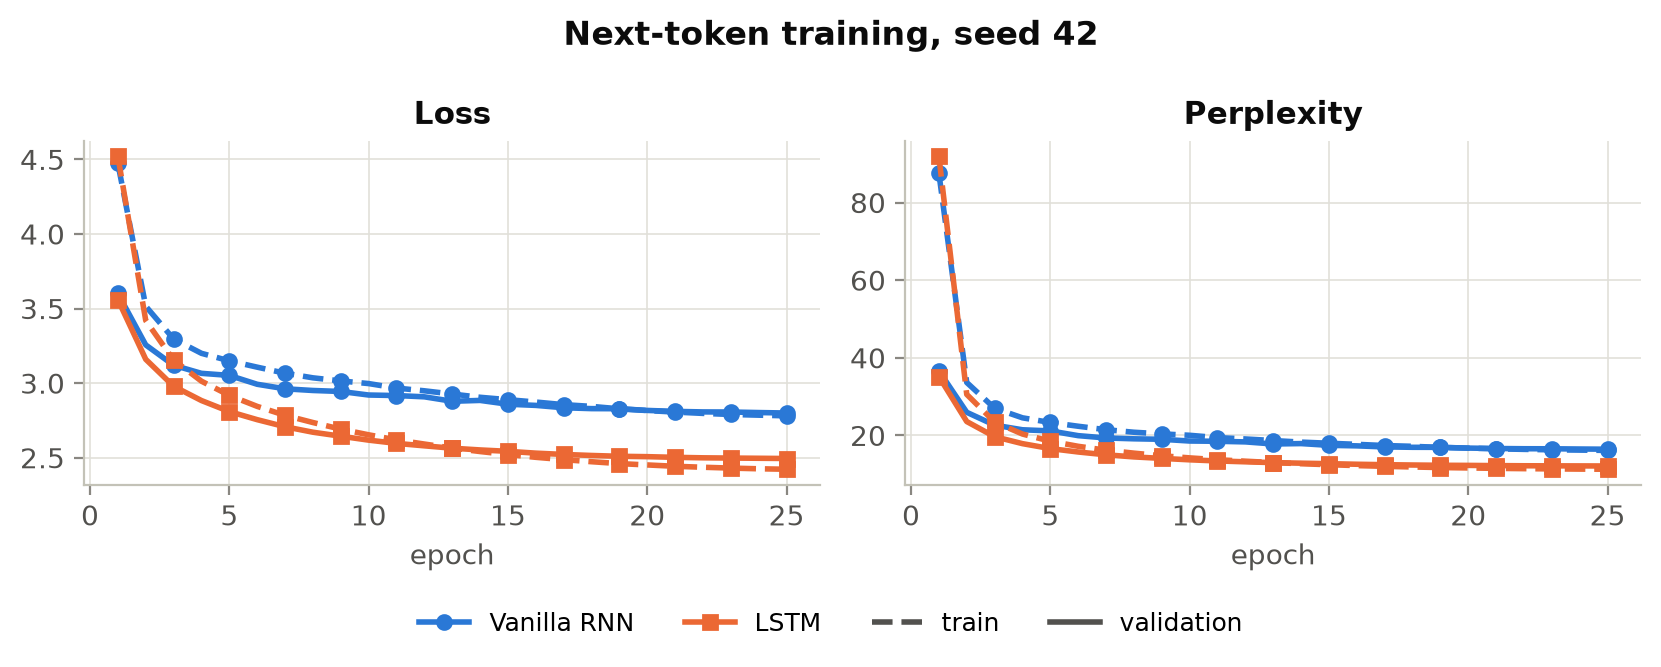
\includegraphics[width=0.95\linewidth,height=0.30\textheight,keepaspectratio]{../outputs/figures/training_curves_seed42.png}
\caption{Training and validation loss and perplexity, seed 42 (RNN and LSTM). Seed 43 is in the repository.}
\end{figure}

The 281-minute training time of the seed-43 RNN is a wall-clock outlier (every other run took 26 to 40 minutes on the same GPU); I did not investigate it (likely other load on the machine), so only the seed-42 times are used in the comparison.

\textbf{Caveat on convergence.} Both models reached the 25-epoch cap (the LSTM seed-43 best epoch is 24), so early
stopping never fired and neither is fully converged. In the final epochs the validation loss was still falling by about
0.003 per epoch while the learning rate had decayed to 1e-4, so I expect the remaining gain to be small (well under 0.05
nats), but I did not run a longer schedule, and I cannot rule out that the gap between the models would narrow or widen.
The train and validation losses stay within 0.02 (RNN) and 0.07 (LSTM) of each other, so overfitting is not the
limiting factor. The LSTM overfits slightly more, which is what I would expect from a bigger model.

\hypertarget{decoding-strategies-part-3}{%
\section{4. Decoding strategies (Part 3)}\label{decoding-strategies-part-3}}

\texttt{common.generate} implements greedy decoding, temperature sampling (0.5, 0.8, 1.2) and top-k sampling (k = 10 and 40, at
temperature 1). \texttt{\textless{}unk\textgreater{}}, \texttt{\textless{}pad\textgreater{}} and \texttt{\textless{}sos\textgreater{}} are never generated. The cap is 250 new tokens. For each of
10 openings, each of the two models and each of the six sampling configurations I generated 3 continuations, plus
one greedy continuation (deterministic), for 320 stories in \texttt{outputs/results/generations\_seed42.jsonl}, unedited.
Five of the openings are the decoding prompts (mystery, discovery, unusual character, a problem to solve, an
unexpected ending) and five are the Plot-Twist openings of Section 5; all ten are in \texttt{plot\_twist/prompts.py}, which was
written before any model was trained or sampled.

Metrics were computed on continuations of 12-token prefixes of the 1,000 test stories (see Section 6.1 for definitions),
mean over models trained with the two seeds (seed-42 tables are in \texttt{quantitative\_tables.md}).

\begin{longtable}[]{@{}
  >{\raggedright\arraybackslash}p{(\columnwidth - 12\tabcolsep) * \real{0.1429}}
  >{\raggedright\arraybackslash}p{(\columnwidth - 12\tabcolsep) * \real{0.1429}}
  >{\raggedright\arraybackslash}p{(\columnwidth - 12\tabcolsep) * \real{0.1429}}
  >{\raggedright\arraybackslash}p{(\columnwidth - 12\tabcolsep) * \real{0.1429}}
  >{\raggedright\arraybackslash}p{(\columnwidth - 12\tabcolsep) * \real{0.1429}}
  >{\raggedright\arraybackslash}p{(\columnwidth - 12\tabcolsep) * \real{0.1429}}
  >{\raggedright\arraybackslash}p{(\columnwidth - 12\tabcolsep) * \real{0.1429}}@{}}
\toprule\noalign{}
\begin{minipage}[b]{\linewidth}\raggedright
decoding
\end{minipage} & \begin{minipage}[b]{\linewidth}\raggedright
RNN repetition
\end{minipage} & \begin{minipage}[b]{\linewidth}\raggedright
LSTM repetition
\end{minipage} & \begin{minipage}[b]{\linewidth}\raggedright
RNN distinct-2
\end{minipage} & \begin{minipage}[b]{\linewidth}\raggedright
LSTM distinct-2
\end{minipage} & \begin{minipage}[b]{\linewidth}\raggedright
RNN too-long
\end{minipage} & \begin{minipage}[b]{\linewidth}\raggedright
LSTM too-long
\end{minipage} \\
\midrule\noalign{}
\endhead
\bottomrule\noalign{}
\endlastfoot
greedy & 0.407 & 0.392 & 0.007 & 0.020 & 43.4\% & 27.1\% \\
temp 0.5 & 0.072 & 0.115 & 0.066 & 0.069 & 5.8\% & 5.3\% \\
temp 0.8 & 0.024 & 0.037 & 0.153 & 0.152 & 11.4\% & 6.9\% \\
temp 1.2 & 0.003 & 0.005 & 0.359 & 0.344 & 19.9\% & 8.8\% \\
top-k 10 & 0.026 & 0.038 & 0.102 & 0.111 & 9.9\% & 8.5\% \\
top-k 40 & 0.014 & 0.022 & 0.158 & 0.166 & 16.3\% & 9.0\% \\
real test stories & 0.045 & & 0.237 & & 8.4\% & \\
\end{longtable}

(Repetition rate = share of word trigrams that are repeats within a story; ``too-long'' = no \texttt{\textless{}eos\textgreater{}} within 250 tokens.
Real stories are measured over the same tail so the comparison is fair.)

\textbf{Do low temperatures repeat?} Yes, but the real problem is greedy decoding. Greedy output is a loop in 41\% (LSTM) and
44\% (RNN) of stories (degenerate share, i.e.~repetition rate at least 0.5), with a repetition rate 9x that of real
text, and Distinct-2 of 0.007 to 0.02 against 0.237 for real text. Typical LSTM greedy output on the detective opening
is ``It was a big, shiny thing.'' repeated until the cap, and the RNN's greedy output on the robot opening is ``He was so
excited! He ran to the edge of the pond and saw a big tree.'' repeated. Temperature 0.5 is much better, but it is
still above human repetition (0.07 and 0.12 against 0.045), so the ``safe'' setting remains repetitive. At 0.8 the
repetition rate is below that of real stories.

\textbf{Do high temperatures become incoherent?} Yes, in a different way from what Distinct-n would suggest. At 1.2
repetition is almost zero (0.3\% to 0.5\%) and Distinct-2 (0.34 to 0.36) is \emph{above} the real text (0.237), which is
the signature of noise rather than of creativity: the model is picking improbable words. Example (RNN, temp 0.8, robot
opening): ``At the end of the day, the worm felt so happy. The little girl was relieved, so she promised himself that she
would fill the bag with water.'' Ungrammatical agreements (``promised himself'', ``what were'') and subject changes
appear already at 0.8, and get worse at 1.2. High temperature also breaks the stopping behaviour: the share of
stories that never end rises from 5.8\% to 19.9\% for the RNN between 0.5 and 1.2, since the model samples
other words in place of \texttt{\textless{}eos\textgreater{}}.

\textbf{Is top-k a useful compromise?} On the metrics, yes. Top-k 40 gives a repetition rate of 0.014 to 0.022 (below real text), Distinct-2 of
0.16, and, unlike temperature 1.2, a normal share of finished stories for the LSTM (9.0\%, about the same as the real 8.4\%). It beats temperature
sampling at an equal level of diversity: top-k 40 and temperature 0.8 have almost the same Distinct-2 (0.16 and 0.15), but top-k cuts off the
unlikely tail that causes the worst words. Qualitatively it is only a modest improvement; the top-k 40 stories above are still disconnected from
the opening. k = 10 trades diversity for safety (Distinct-2 0.10 to 0.11, repetition 0.03) and sits between 0.5 and 0.8.
My recommendation for this model would be top-k 40, or temperature 0.8, never greedy.

Figures: \texttt{outputs/figures/decoding\_*\_seed42.png} and \texttt{...\_seed43.png}.

\begin{figure}[htbp]
\centering
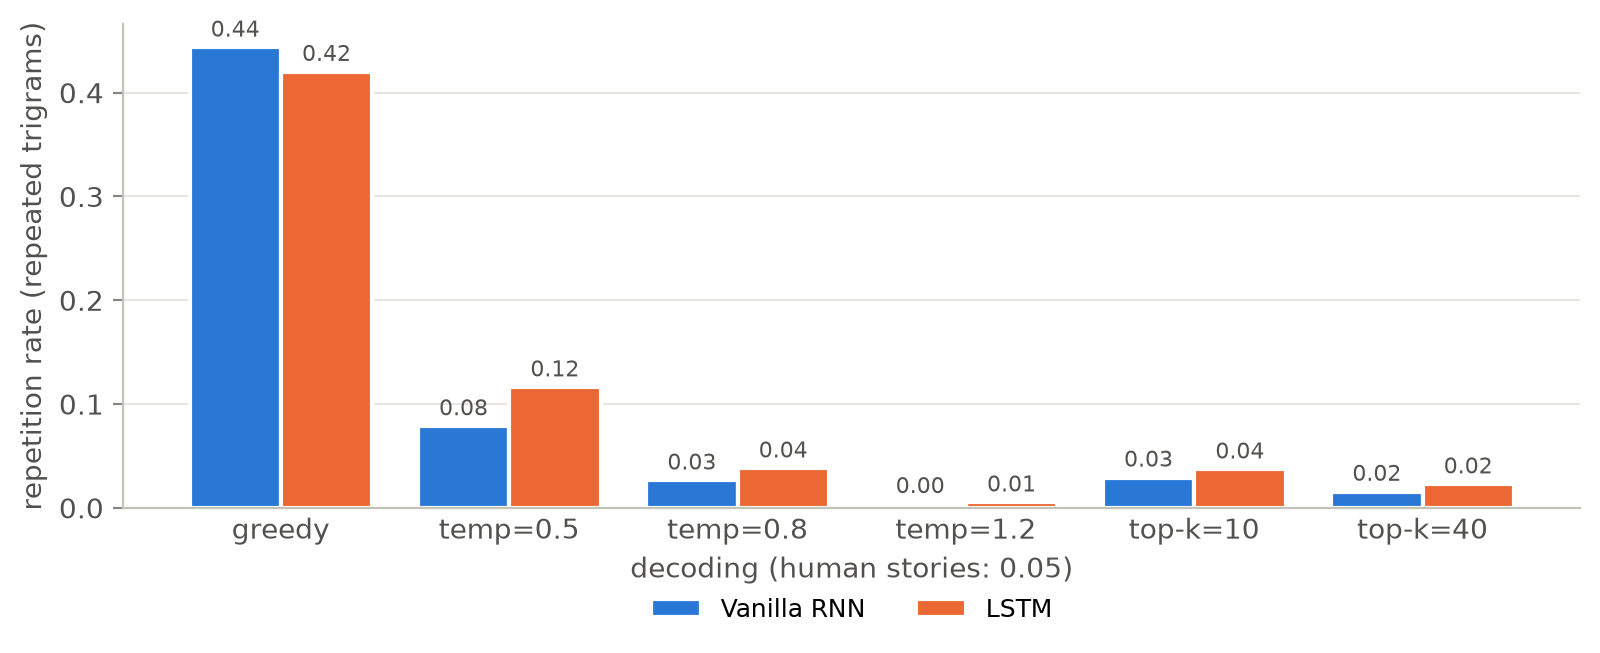
\includegraphics[width=0.49\linewidth,height=0.30\textheight,keepaspectratio]{../outputs/figures/decoding_repetition_rate_seed42.png}\hfill
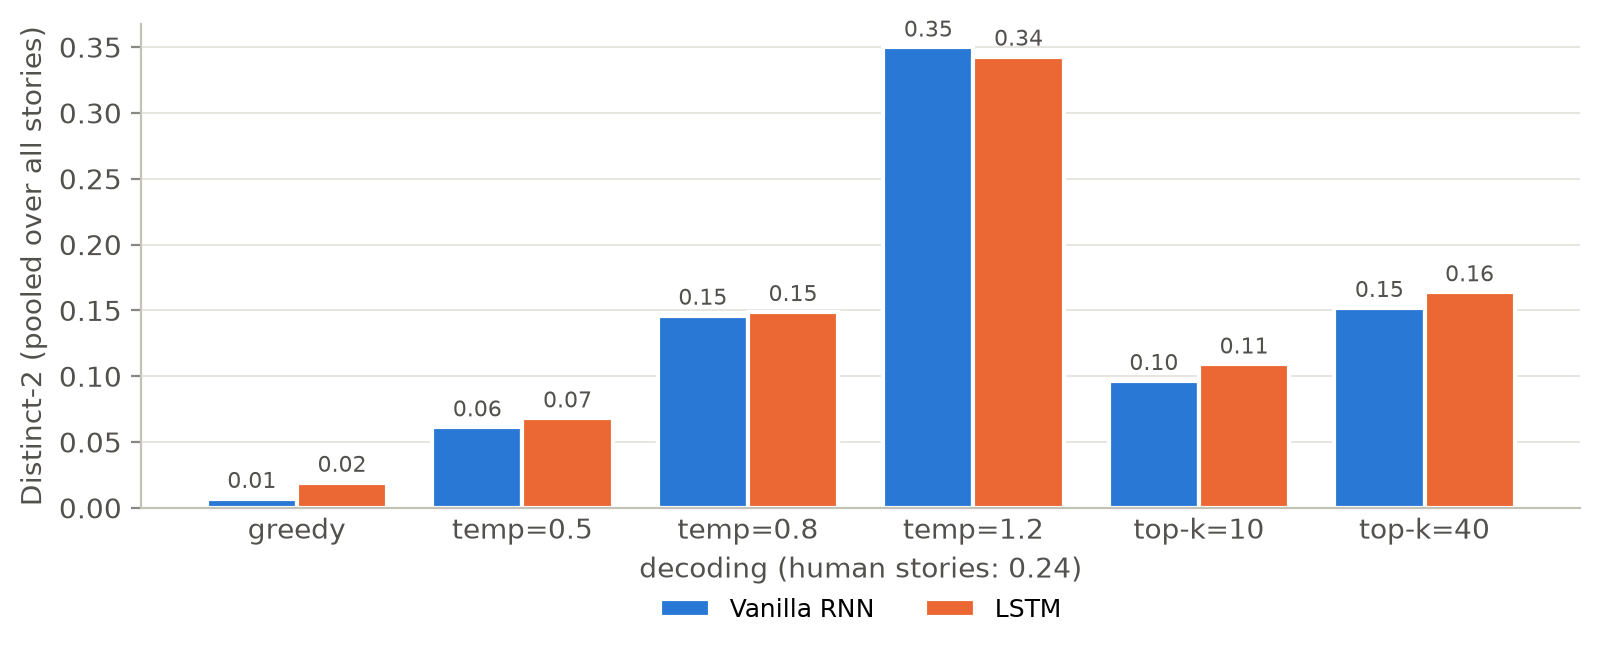
\includegraphics[width=0.49\linewidth,height=0.30\textheight,keepaspectratio]{../outputs/figures/decoding_distinct_2_seed42.png}
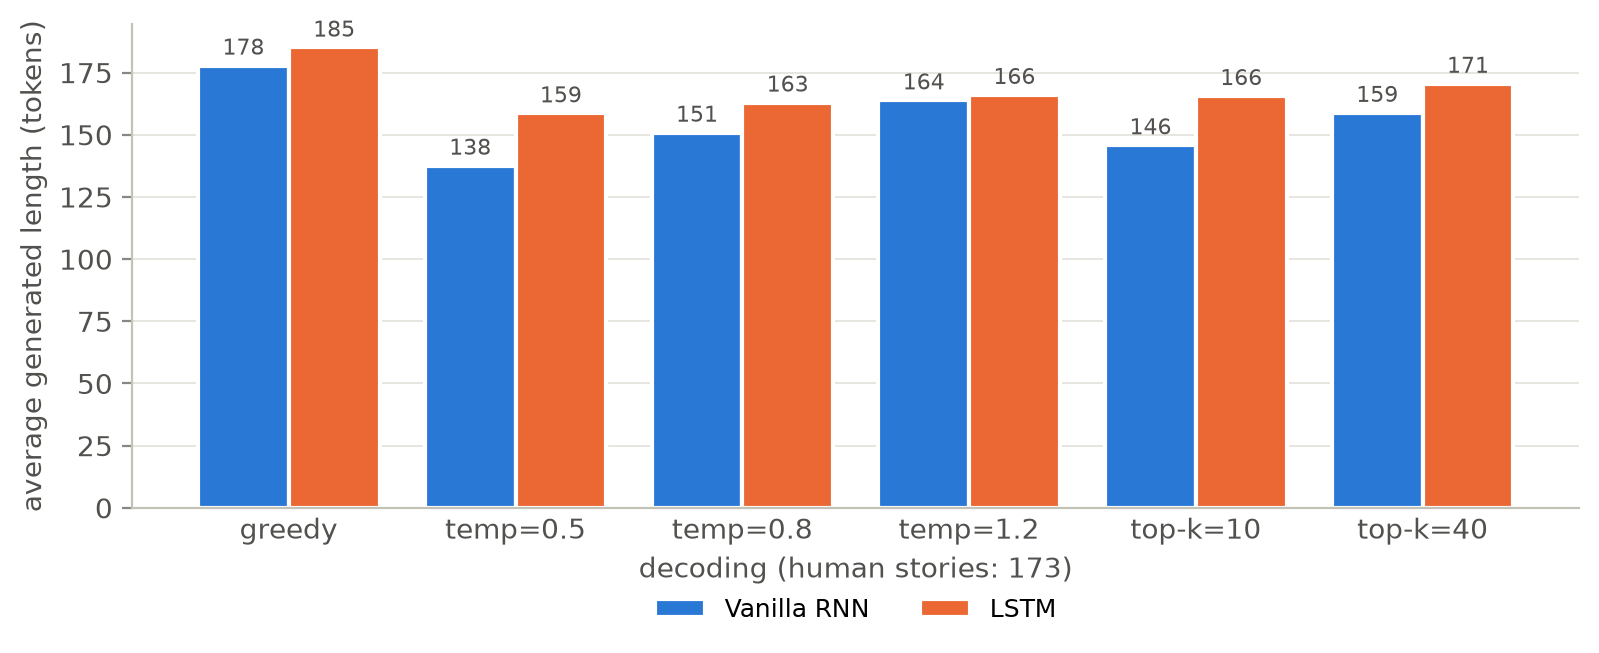
\includegraphics[width=0.49\linewidth,height=0.30\textheight,keepaspectratio]{../outputs/figures/decoding_avg_length_seed42.png}\hfill
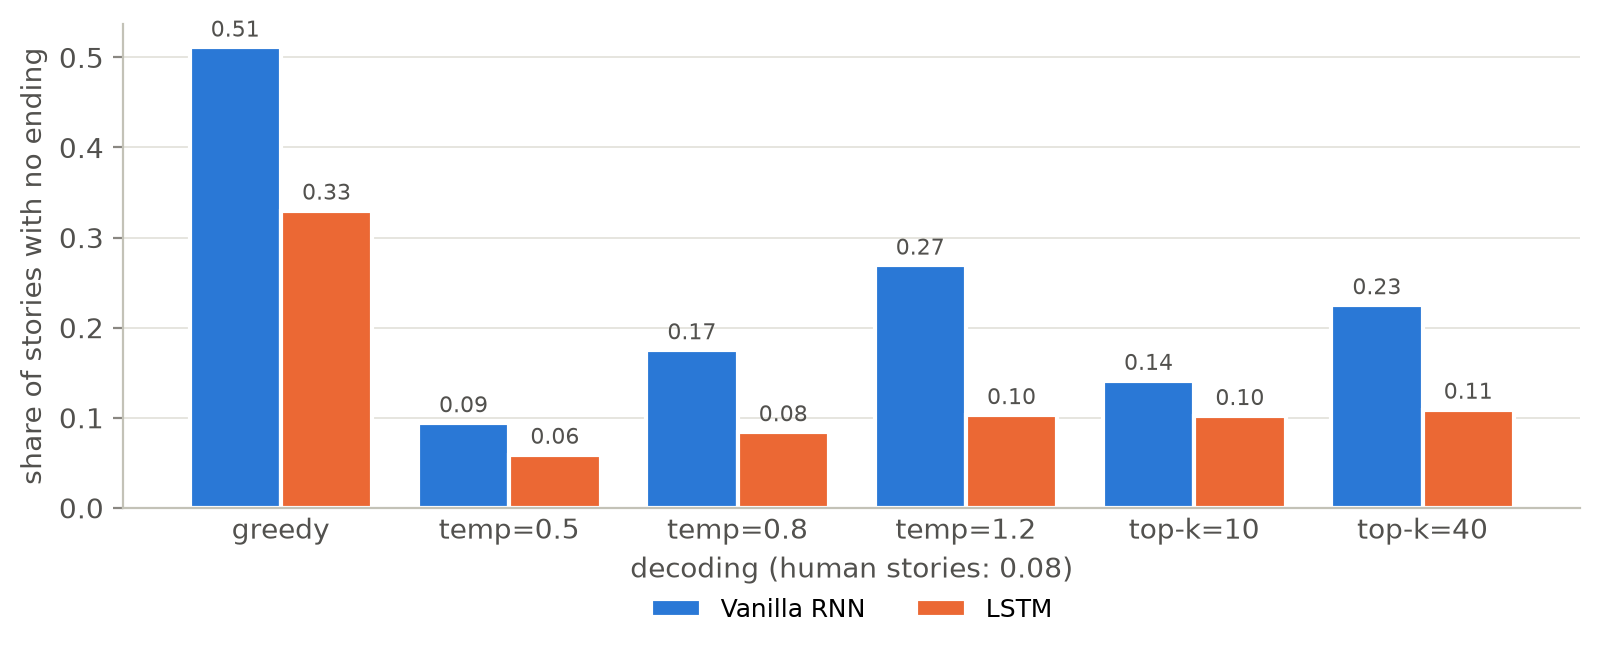
\includegraphics[width=0.49\linewidth,height=0.30\textheight,keepaspectratio]{../outputs/figures/decoding_too_long_share_seed42.png}
\caption{Decoding comparison, seed 42: repetition rate, Distinct-2, average length and share of stories that never end, per decoding configuration and model.}
\end{figure}

\hypertarget{the-plot-twist-challenge-part-4}{%
\section{5. The Plot-Twist Challenge (Part 4)}\label{the-plot-twist-challenge-part-4}}

The five openings (\texttt{plot\_twist/prompts.py}) rewrite the brief's examples in the register of the corpus, since the models
have only seen TinyStories: a test paper that already has tomorrow's answers; an old robot receiving a message from his
future self; a detective in a house where every clock stopped at midnight and the phone rings; a village that
wakes up having forgotten yesterday; a letter written one hundred years in the future. Each was run with both
models under all six sampling configurations (3 samples each) and with greedy decoding, so every opening has more than the required
two decoding strategies for each model. Generated text is not edited anywhere. Full text:
\texttt{outputs/results/generated\_stories\_seed42.md}; the generations are in \texttt{generations\_seed42.jsonl}.

\hypertarget{automatic-evidence-for-the-four-criteria}{%
\subsection{5.1 Automatic evidence for the four criteria}\label{automatic-evidence-for-the-four-criteria}}

\texttt{analyze\_plot\_twist.py} measures proxies (definitions are in the script and in \texttt{plot\_twist\_proxies.md}):
prompt coverage (share of the opening's content words that the continuation reuses), new content words, repetition,
and the share of continuations that keep a character named in the opening.

\begin{longtable}[]{@{}
  >{\raggedright\arraybackslash}p{(\columnwidth - 12\tabcolsep) * \real{0.1429}}
  >{\raggedright\arraybackslash}p{(\columnwidth - 12\tabcolsep) * \real{0.1429}}
  >{\raggedright\arraybackslash}p{(\columnwidth - 12\tabcolsep) * \real{0.1429}}
  >{\raggedright\arraybackslash}p{(\columnwidth - 12\tabcolsep) * \real{0.1429}}
  >{\raggedright\arraybackslash}p{(\columnwidth - 12\tabcolsep) * \real{0.1429}}
  >{\raggedright\arraybackslash}p{(\columnwidth - 12\tabcolsep) * \real{0.1429}}
  >{\raggedright\arraybackslash}p{(\columnwidth - 12\tabcolsep) * \real{0.1429}}@{}}
\toprule\noalign{}
\begin{minipage}[b]{\linewidth}\raggedright
model
\end{minipage} & \begin{minipage}[b]{\linewidth}\raggedright
decoding
\end{minipage} & \begin{minipage}[b]{\linewidth}\raggedright
prompt coverage
\end{minipage} & \begin{minipage}[b]{\linewidth}\raggedright
new content words
\end{minipage} & \begin{minipage}[b]{\linewidth}\raggedright
repetition
\end{minipage} & \begin{minipage}[b]{\linewidth}\raggedright
name kept
\end{minipage} & \begin{minipage}[b]{\linewidth}\raggedright
ended
\end{minipage} \\
\midrule\noalign{}
\endhead
\bottomrule\noalign{}
\endlastfoot
LSTM & greedy & 0.12 & 13.8 & 0.52 & 0.50 & 0.80 \\
LSTM & temp 0.8 & 0.09 & 34.7 & 0.02 & 0.67 & 1.00 \\
LSTM & top-k 40 & 0.10 & 40.3 & 0.01 & 0.50 & 1.00 \\
RNN & greedy & 0.00 & 12.8 & 0.30 & 0.00 & 0.80 \\
RNN & temp 0.8 & 0.06 & 37.1 & 0.02 & 0.00 & 1.00 \\
RNN & top-k 40 & 0.05 & 48.9 & 0.01 & 0.00 & 0.87 \\
\end{longtable}

``Name kept'' is only defined for the two openings with a named character (Sara, Jack), so each cell is based on a few stories and
should be read as indicative only.

\hypertarget{my-assessment-human-commentary-separate-from-the-generated-text}{%
\subsection{5.2 My assessment (human commentary, separate from the generated text)}\label{my-assessment-human-commentary-separate-from-the-generated-text}}

Judged against the four criteria, on the stories I read (the first sample for every opening, model and the
greedy / temperature 0.8 / top-k 40 settings, 30 stories; also the full set by the proxies above):

\begin{enumerate}
\def\labelenumi{\arabic{enumi}.}
\tightlist
\item
  \textbf{Connection to the prompt: poor for both models, slightly better for the LSTM.} Prompt coverage is at most 0.12 for any configuration, and in nearly every
  story the continuation could follow any TinyStories opening. The strongest connection I found was LSTM
  on the letter opening (``Jack was so happy to have found the letter \ldots{} put it in his pocket''), and with greedy decoding on the
  exam opening (``Sara'' is never mentioned, but ``she'' is). The RNN kept a named character in none of the stories
  (0.00 in every setting) and drifted to unrelated characters (``Tommy and his cat'', ``Bob'', ``Lily''). The LSTM
  also drifts (the exam opening continues with ``Lily'', ``Anna'', ``Mia'') but anchors on the opening's name more often.
\item
  \textbf{A meaningful development or twist: not found.} Across the 30 stories I read, none contained a reveal or
  reversal that the opening sets up. The time-travel, stopped clocks, and forgotten-day premises are never picked up:
  no story mentions a clock, a message from the future, or forgetting. What the models produce is the generic
  TinyStories arc (a character becomes happy, meets a friend, learns a lesson). The nearest thing to ``surprise'' is
  random noise, e.g.~the LSTM's detective continuation at temp 0.8, in which ``a big, scary monster'' appears and then the
  man says ``I just wanted to go home now'', which is not connected to the opening and which no reader would call a twist.
  The `new content words' column shows the same thing: high values at temp 1.2 (53 to 66) are a consequence of randomness, not of plot.
\item
  \textbf{Consistency with details established earlier: weak.} Within a story, names and objects change: the LSTM's exam story at top-k
  40 begins with ``Sara'' and then ``Lily and her mother went to the house'', ``Mia's bed''. The RNN's top-k 40 robot story
  goes through ``Sam'', ``John'', ``Timmy''. Pronouns flip between ``he'' and ``she'' for the same character. Greedy output is the only
  consistent output, and only because it repeats one sentence.
\item
  \textbf{Repetition and abrupt transitions: greedy fails, sampling mostly avoids repetition but is abrupt.} Greedy output is a loop (repetition rate at least 0.5) in 1 of 5 (RNN)
  and 2 of 5 (LSTM) of the Plot-Twist greedy stories, and the others contain repeated sentences. For sampled output,
  repetition is gone but the transitions are the problem: ``The librarian said \ldots{} Sara thought for a moment \ldots{} Lily and her mother went to the
  house \ldots{} saw a big box of ash on the wall, so he had to wait.'' (LSTM, top-k 40) is grammatical sentence by sentence and has no thread.
\end{enumerate}

\textbf{Comparing the two models.} The LSTM's stories are a bit longer, end more reliably (at temperature 0.8 and top-k 40, 30 of 30 sampled twist stories ended
for the LSTM against 28 of 30 for the RNN; at temperature 1.2 only 67\% of the RNN's did, against 100\%), keep names more often, and are more fluent sentence by sentence.
In my own reading the RNN's sentences had more grammatical errors (``what that were'', ``promised himself'', ``so so he went''), but the blinded raters scored the RNN's grammar \emph{higher} (4.08 against 3.83; Section 6.3, difference not significant), so I do not rely on my impression here. Neither produced
a story I would call coherent, and the difference between them is smaller than the difference between greedy and sampled output.

\hypertarget{optional-extension-a-small-open-source-llm}{%
\subsection{5.3 Optional extension: a small open-source LLM}\label{optional-extension-a-small-open-source-llm}}

I evaluated \texttt{HuggingFaceTB/SmolLM2-360M-Instruct}, \textbf{zero-shot, no fine-tuning}, on the same ten openings, as the
brief allows. Exact settings are in \texttt{outputs/results/llm\_settings.json}: system prompt ``You are a children's story writer.'', the user prompt
``Here is the beginning of a short story for young children. Continue the story in simple language and give it an ending.
Write only the continuation, in plain text.\n\nBeginning: \{opening\}'', fp16, GTX 1650, 250 new (sub-word) tokens, greedy, temperature 0.8 and
top-k 40. Its outputs are in \texttt{outputs/results/llm\_generations.jsonl}.

\begin{longtable}[]{@{}
  >{\raggedright\arraybackslash}p{(\columnwidth - 10\tabcolsep) * \real{0.1667}}
  >{\raggedright\arraybackslash}p{(\columnwidth - 10\tabcolsep) * \real{0.1667}}
  >{\raggedright\arraybackslash}p{(\columnwidth - 10\tabcolsep) * \real{0.1667}}
  >{\raggedright\arraybackslash}p{(\columnwidth - 10\tabcolsep) * \real{0.1667}}
  >{\raggedright\arraybackslash}p{(\columnwidth - 10\tabcolsep) * \real{0.1667}}
  >{\raggedright\arraybackslash}p{(\columnwidth - 10\tabcolsep) * \real{0.1667}}@{}}
\toprule\noalign{}
\begin{minipage}[b]{\linewidth}\raggedright
model
\end{minipage} & \begin{minipage}[b]{\linewidth}\raggedright
decoding
\end{minipage} & \begin{minipage}[b]{\linewidth}\raggedright
distinct-2 (all samples)
\end{minipage} & \begin{minipage}[b]{\linewidth}\raggedright
repetition
\end{minipage} & \begin{minipage}[b]{\linewidth}\raggedright
too long
\end{minipage} & \begin{minipage}[b]{\linewidth}\raggedright
avg length
\end{minipage} \\
\midrule\noalign{}
\endhead
\bottomrule\noalign{}
\endlastfoot
RNN & temp 0.8 & 0.554 & 0.022 & 6.7\% & 120 \\
LSTM & temp 0.8 & 0.553 & 0.028 & 6.7\% & 130 \\
SmolLM2-360M & temp 0.8 & 0.610 & 0.037 & 46.7\% & 157 \\
RNN & greedy & 0.186 & 0.428 & 40\% & 141 \\
LSTM & greedy & 0.253 & 0.482 & 20\% & 157 \\
SmolLM2-360M & greedy & 0.551 & 0.170 & 50\% & 175 \\
\end{longtable}

These are the ten openings, so each cell is based on 10 to 30 stories. The LLM loops far less under greedy decoding
(repetition 0.17 against 0.43 to 0.48 and no degenerate stories), which is expected from a model trained on far more text.
Its ``too long'' share counts sub-word tokens against a cap of 250, which is not the same unit as for the word-level models, so that column is not
directly comparable. Its stories are not human-rated, so I make no quality claim beyond these metrics. Perplexity is not
compared because the tokenisers differ.

\hypertarget{evaluation-the-better-language-model-and-the-better-storyteller-part-5}{%
\section{6. Evaluation: the better language model and the better storyteller (Part 5)}\label{evaluation-the-better-language-model-and-the-better-storyteller-part-5}}

\hypertarget{quantitative-evaluation}{%
\subsection{6.1 Quantitative evaluation}\label{quantitative-evaluation}}

\textbf{Perplexity} is exp of the mean next-token cross-entropy over real (non-pad) target tokens, in fp32, on the same
held-out splits for both models (vocabulary of 6,534, the same for both).

\begin{longtable}[]{@{}llll@{}}
\toprule\noalign{}
model & val ppl & test ppl & test ppl, 2 seeds \\
\midrule\noalign{}
\endhead
\bottomrule\noalign{}
\endlastfoot
Vanilla RNN & 16.44 & 16.15 & 16.14 \ensuremath{\pm} 0.02 \\
LSTM & 12.12 & 11.86 & 11.79 \ensuremath{\pm} 0.09 \\
\end{longtable}

\textbf{Generation settings.} For each of the 1,000 test stories, the first 12 tokens are given as the opening and the
model continues with a cap of 250 new tokens, for each of the six decoding configurations, so all metrics use the
same held-out split (\texttt{generation\_settings\_seed42.json} records the settings and seeds).

\textbf{Metric definitions.}
- \emph{Distinct-1 / Distinct-2}: number of unique unigrams / bigrams divided by the total, pooled over a group of
generated stories (corpus-level; \texttt{\_story} columns are the average per story). Corpus-level Distinct is only
comparable between groups with the same amount of text.
- \emph{Repetition rate}: the share of word trigrams in a story that are repeats of an earlier trigram in the same story
(0 = none, close to 1 = a loop). A story with a rate of at least 0.5 is counted as \emph{degenerate}.
- \emph{Length}: average number of generated tokens; \emph{too short} = the story ended with \texttt{\textless{}eos\textgreater{}} after fewer than 30 tokens;
\emph{too long} = no \texttt{\textless{}eos\textgreater{}} within the 250-token cap.

The complete tables (every decoding configuration, both seeds, and the real test stories as a reference) are in
\texttt{outputs/results/quantitative\_tables.md}; the decoding comparison is in Section 4. Across all configurations the RNN and LSTM
are close on Distinct-1 and Distinct-2 (differences of at most 0.03), so diversity does not separate them. What does separate
them is repetition at a fixed temperature (the RNN is lower: 0.072 against 0.115 at 0.5), per-story diversity
(RNN higher), and stopping behaviour (the LSTM ends far more reliably: 8.8\% against 19.9\% never-ending at 1.2).
Premature termination is rare (below 2\% everywhere). The metrics were stable between the two training seeds.

\hypertarget{human-evaluation-setup}{%
\subsection{6.2 Human evaluation setup}\label{human-evaluation-setup}}

\texttt{build\_human\_eval.py} builds a blinded set of \textbf{20 samples}: the five Plot-Twist openings, 2 models, 2 decodings (greedy and
top-k 40), the first sample of each, shuffled with seed 2024 and given neutral ids S01 to S20. The private answer key (\texttt{key.json}) maps ids back to model
and decoding and is not shown to raters. Each sample is rated 1 to 5 for \textbf{coherence, grammatical quality, relevance
to the opening, and creativity/surprise} in \texttt{outputs/human\_eval/rate.html}, a self-contained form that downloads a CSV. Samples are
shown as generated, with no editing. Four raters returned complete ratings (80 ratings in total, 20 stories each). Raters are my group members, who knew the
assignment but were not told which model wrote which story; they were instructed not to look at the generations or this report before rating, and the author confirms that the rating was done blind (this is the author's confirmation, not something the analysis can check).

\hypertarget{human-results}{%
\subsection{6.3 Human results}\label{human-results}}

All tables are produced by \texttt{analyze\_human\_eval.py} (\texttt{outputs/results/human\_eval\_tables.md}, \texttt{human\_eval.json}) and the figure is
\texttt{outputs/figures/human\_ratings.png}.

\begin{figure}[htbp]
\centering
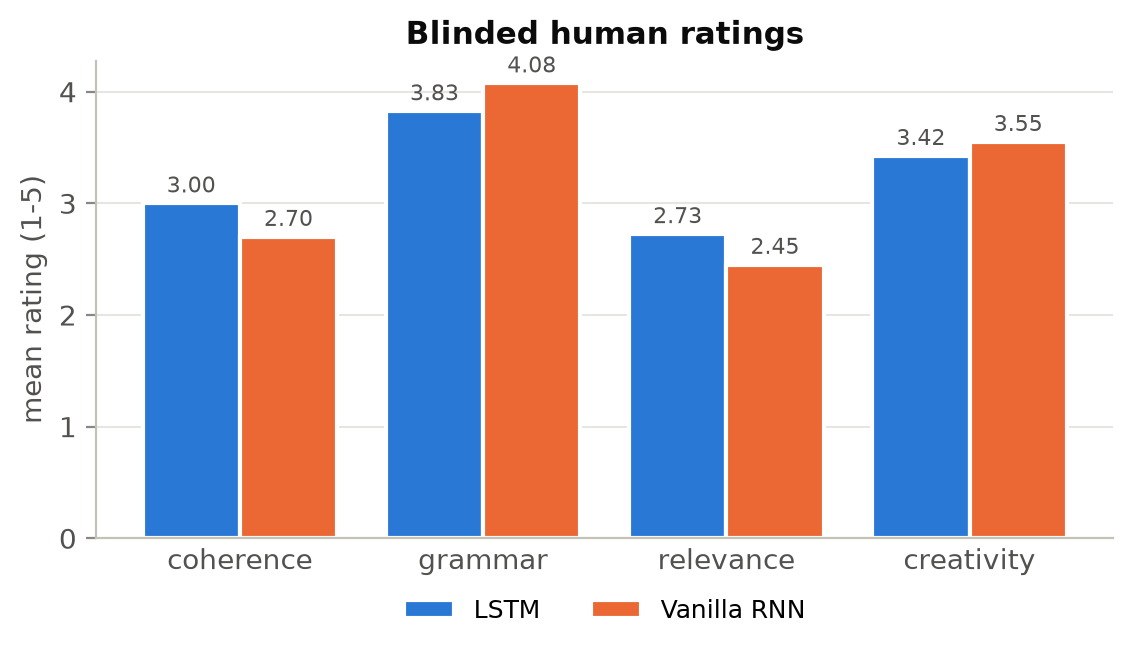
\includegraphics[width=0.8\linewidth,height=0.30\textheight,keepaspectratio]{../outputs/figures/human_ratings.png}
\caption{Mean blinded human ratings per model and criterion.}
\end{figure}

Each story's score is the mean over raters; the table gives the mean \ensuremath{\pm} standard deviation across the 10 stories per model.

\textbf{Mean rating by model (1 to 5).}

\begin{longtable}[]{@{}
  >{\raggedright\arraybackslash}p{(\columnwidth - 12\tabcolsep) * \real{0.1429}}
  >{\raggedright\arraybackslash}p{(\columnwidth - 12\tabcolsep) * \real{0.1429}}
  >{\raggedright\arraybackslash}p{(\columnwidth - 12\tabcolsep) * \real{0.1429}}
  >{\raggedright\arraybackslash}p{(\columnwidth - 12\tabcolsep) * \real{0.1429}}
  >{\raggedright\arraybackslash}p{(\columnwidth - 12\tabcolsep) * \real{0.1429}}
  >{\raggedright\arraybackslash}p{(\columnwidth - 12\tabcolsep) * \real{0.1429}}
  >{\raggedright\arraybackslash}p{(\columnwidth - 12\tabcolsep) * \real{0.1429}}@{}}
\toprule\noalign{}
\begin{minipage}[b]{\linewidth}\raggedright
model
\end{minipage} & \begin{minipage}[b]{\linewidth}\raggedright
coherence
\end{minipage} & \begin{minipage}[b]{\linewidth}\raggedright
grammar
\end{minipage} & \begin{minipage}[b]{\linewidth}\raggedright
relevance
\end{minipage} & \begin{minipage}[b]{\linewidth}\raggedright
creativity
\end{minipage} & \begin{minipage}[b]{\linewidth}\raggedright
overall
\end{minipage} & \begin{minipage}[b]{\linewidth}\raggedright
val ppl
\end{minipage} \\
\midrule\noalign{}
\endhead
\bottomrule\noalign{}
\endlastfoot
LSTM & 3.00 \ensuremath{\pm} 0.57 & 3.83 \ensuremath{\pm} 0.43 & 2.73 \ensuremath{\pm} 0.52 & 3.42 \ensuremath{\pm} 0.59 & 3.24 & 12.12 \\
Vanilla RNN & 2.70 \ensuremath{\pm} 0.51 & 4.08 \ensuremath{\pm} 0.39 & 2.45 \ensuremath{\pm} 0.52 & 3.55 \ensuremath{\pm} 0.52 & 3.19 & 16.44 \\
\end{longtable}

\textbf{By decoding configuration (5 stories each).}

\begin{longtable}[]{@{}
  >{\raggedright\arraybackslash}p{(\columnwidth - 12\tabcolsep) * \real{0.1429}}
  >{\raggedright\arraybackslash}p{(\columnwidth - 12\tabcolsep) * \real{0.1429}}
  >{\raggedright\arraybackslash}p{(\columnwidth - 12\tabcolsep) * \real{0.1429}}
  >{\raggedright\arraybackslash}p{(\columnwidth - 12\tabcolsep) * \real{0.1429}}
  >{\raggedright\arraybackslash}p{(\columnwidth - 12\tabcolsep) * \real{0.1429}}
  >{\raggedright\arraybackslash}p{(\columnwidth - 12\tabcolsep) * \real{0.1429}}
  >{\raggedright\arraybackslash}p{(\columnwidth - 12\tabcolsep) * \real{0.1429}}@{}}
\toprule\noalign{}
\begin{minipage}[b]{\linewidth}\raggedright
model
\end{minipage} & \begin{minipage}[b]{\linewidth}\raggedright
decoding
\end{minipage} & \begin{minipage}[b]{\linewidth}\raggedright
coherence
\end{minipage} & \begin{minipage}[b]{\linewidth}\raggedright
grammar
\end{minipage} & \begin{minipage}[b]{\linewidth}\raggedright
relevance
\end{minipage} & \begin{minipage}[b]{\linewidth}\raggedright
creativity
\end{minipage} & \begin{minipage}[b]{\linewidth}\raggedright
overall
\end{minipage} \\
\midrule\noalign{}
\endhead
\bottomrule\noalign{}
\endlastfoot
LSTM & greedy & 3.10 & 3.95 & 2.70 & 3.10 & 3.21 \\
LSTM & top-k 40 & 2.90 & 3.70 & 2.75 & 3.75 & 3.27 \\
RNN & greedy & 2.95 & 4.05 & 2.45 & 3.25 & 3.17 \\
RNN & top-k 40 & 2.45 & 4.10 & 2.45 & 3.85 & 3.21 \\
\end{longtable}

\textbf{Paired comparison, LSTM minus RNN} (10 matched pairs: same opening, same decoding; bootstrap CI over the pairs).

\begin{longtable}[]{@{}llll@{}}
\toprule\noalign{}
criterion & mean diff & 95\% CI & LSTM wins / ties / RNN wins \\
\midrule\noalign{}
\endhead
\bottomrule\noalign{}
\endlastfoot
coherence & +0.30 & {[}-0.23, +0.78{]} & 6 / 1 / 3 \\
grammar & -0.25 & {[}-0.57, +0.03{]} & 1 / 4 / 5 \\
relevance & +0.28 & {[}-0.15, +0.80{]} & 5 / 4 / 1 \\
creativity & -0.12 & {[}-0.38, +0.15{]} & 3 / 1 / 6 \\
overall & +0.05 & {[}-0.22, +0.36{]} & 4 / 1 / 5 \\
\end{longtable}

Every interval contains zero. With only 10 pairs the study cannot separate the models; the signs are suggestive, not established.

\textbf{Inter-rater agreement.}

\begin{longtable}[]{@{}
  >{\raggedright\arraybackslash}p{(\columnwidth - 8\tabcolsep) * \real{0.2000}}
  >{\raggedright\arraybackslash}p{(\columnwidth - 8\tabcolsep) * \real{0.2000}}
  >{\raggedright\arraybackslash}p{(\columnwidth - 8\tabcolsep) * \real{0.2000}}
  >{\raggedright\arraybackslash}p{(\columnwidth - 8\tabcolsep) * \real{0.2000}}
  >{\raggedright\arraybackslash}p{(\columnwidth - 8\tabcolsep) * \real{0.2000}}@{}}
\toprule\noalign{}
\begin{minipage}[b]{\linewidth}\raggedright
criterion
\end{minipage} & \begin{minipage}[b]{\linewidth}\raggedright
Krippendorff alpha (ordinal)
\end{minipage} & \begin{minipage}[b]{\linewidth}\raggedright
mean pairwise weighted kappa
\end{minipage} & \begin{minipage}[b]{\linewidth}\raggedright
exact agreement
\end{minipage} & \begin{minipage}[b]{\linewidth}\raggedright
within 1 point
\end{minipage} \\
\midrule\noalign{}
\endhead
\bottomrule\noalign{}
\endlastfoot
coherence & -0.14 & 0.01 & 25\% & 48\% \\
grammar & -0.14 & -0.06 & 21\% & 62\% \\
relevance & -0.17 & 0.05 & 15\% & 46\% \\
creativity & -0.14 & 0.02 & 26\% & 58\% \\
\end{longtable}

\begin{longtable}[]{@{}lllll@{}}
\toprule\noalign{}
rater & coherence & grammar & relevance & creativity \\
\midrule\noalign{}
\endhead
\bottomrule\noalign{}
\endlastfoot
Ayush & 4.40 & 4.70 & 4.35 & 4.60 \\
Keshav & 2.15 & 3.65 & 1.25 & 2.50 \\
Rishi Kharya & 2.15 & 4.65 & 2.10 & 3.70 \\
Shivam Singh & 2.70 & 2.80 & 2.65 & 3.15 \\
\end{longtable}

\textbf{Disagreement between evaluators.} Agreement is essentially nil (alpha between -0.17 and -0.14, kappa about 0), so the individual story
means rest on four mostly unrelated opinions, and I treat the averages as weak evidence. Two things drive it:
- \emph{Different use of the scale.} Ayush rated almost everything 4 or 5 on all criteria (mean 4.4 to 4.7), while Keshav gave relevance 1 to 17 of 20
stories (mean 1.25), and Shivam used the full range. Ayush gave the maximum score on all four criteria to the pure loop S01 (one sentence, ``It was a big, shiny
thing.'', repeated about 25 times) and to the unfinished RNN loop S08, both of which Shivam scored all 1s; that is a 4-point spread on the same text, and suggests that Ayush's
ratings do not discriminate between good and bad outputs. I kept his ratings in the main tables (I have no ground to exclude a rater after seeing results), but report
the sensitivity below.
- \emph{Different criteria.} Raters disagree about what ``relevance'' and ``creativity'' reward. Keshav, who judged relevance harshly, still gave 5 on coherence to S11, S12 and S15, which are
fluent but unrelated to the opening, so he appears to separate coherence from relevance more than the others, while Rishi Kharya's grammar scores (4 to 5 almost throughout) seem to grade
sentence-level fluency only.

\textbf{Sensitivity: without Ayush} (three raters). The conclusions do not change. Overall LSTM 2.84 against RNN 2.73 (paired difference +0.11, CI {[}-0.30, +0.56{]}); coherence
+0.53 (CI {[}-0.17, +1.17{]}, LSTM better in 7 pairs, RNN in 2); grammar -0.33 (CI {[}-0.80, +0.13{]}); relevance +0.33 (CI {[}-0.23, +0.97{]}); creativity -0.10. All intervals still include zero.
Agreement among the remaining three is still near zero (alpha 0.09 coherence, -0.19 grammar, -0.11 relevance, -0.03 creativity), so Ayush alone does not explain the disagreement.

\textbf{What the raters preferred.} The highest-rated stories (mean 3.94) were two short, fluent, generic greedy outputs that ended after a few sentences: S15 (RNN, exam opening, ``She was so happy and she thanked her mom for
helping her\ldots{}'') and S17 (LSTM, letter opening, which keeps the name Jack). The lowest-rated (2.81 to 2.88) included the looping S01 and the unfinished RNN loop S08, together with S03, S11 and S18. Greedy
decoding scored better on coherence than top-k 40 for both models (RNN 2.95 against 2.45, LSTM 3.10 against 2.90), and top-k 40 scored higher on creativity
(RNN 3.85 against 3.25, LSTM 3.75 against 3.10), with the overall score nearly equal (3.17 to 3.27). The raters therefore reward the creativity of sampled text and the coherence of greedy
text about equally, and the loop-prone greedy output was not punished as much as the automatic repetition metric would suggest (one or two of the five stories in each greedy group is a loop, so this rests on very few stories).

\textbf{Perplexity against human judgement.} The LSTM has the lower perplexity (12.1 against 16.4). It scores higher on coherence and relevance, the two criteria that depend most on the model
using context, and lower on grammar and creativity, and its overall rating is the same within noise (+0.05, CI {[}-0.22, +0.36{]}; 4 pairs LSTM, 1 tie, 5 pairs RNN). So in this experiment a 27\% lower perplexity did \textbf{not}
produce a measurably better storyteller.

\hypertarget{final-analysis-part-6}{%
\section{7. Final analysis (Part 6)}\label{final-analysis-part-6}}

\textbf{1. How do the RNN and LSTM differ in their ability to model sequential text?} The LSTM models text better by a clear
margin: test perplexity 11.8 against 16.1 (consistent across two seeds, standard deviations 0.09 and 0.02), at the cost of 22\% more parameters and 1.5x the training time.
The behavioural differences are consistent with better use of context: LSTM stories end properly more often (never-ending share 8.8\% against
19.9\% at temperature 1.2, 27\% against 43\% under greedy) and keep named characters more often in the Plot-Twist stories (0.5 to 0.67 against 0.00). The
caveats are that the LSTM has more parameters, that neither model finished converging within 25 epochs, and that the name statistic comes from
two openings. Both models still fail to keep track of a character across a paragraph.

\textbf{2. Which model generates more coherent and less repetitive continuations?} The LSTM is somewhat more coherent in my reading (fluent sentences,
more consistent names, finishing), and the human raters give the LSTM higher coherence (3.00 against 2.70) and relevance (2.73 against 2.45), though not significantly (CIs include zero) and with near-zero rater agreement; they rate the RNN's grammar higher (4.08 against 3.83). It is \emph{not} less repetitive: at temperature 0.5, 0.8 and in top-k it repeats trigrams 20\% to 60\%
more than the RNN (0.115 against 0.072, 0.037 against 0.024), and in greedy mode the two are within noise (0.42 and 0.44). The likely reason is that a
sharper, better-fitted distribution gives its top choice more of the mass, which makes loops more likely when the choice is made by the argmax or at low temperature. I did not test that explanation directly.

\textbf{3. How does temperature affect creativity and grammatical quality?} Raising the temperature trades repetition for noise. From 0.5 to 1.2,
repetition falls from 0.07/0.12 to 0.003/0.005 and Distinct-2 rises from 0.07 to 0.35, which exceeds that of real text (0.237), meaning that the diversity at 1.2
is partly noise. In my reading, grammar and coherence degrade over the same range: agreement errors and abrupt subject changes
are visible at 0.8 and frequent at 1.2, and stories that never end rise from 6\% to 20\% (RNN). I did not find that any temperature produces \emph{creative}
stories rather than only different ones. The human ratings cover only greedy and top-k 40, not individual temperatures, so they do not test this directly; they do show that top-k 40 samples were rated more creative than greedy ones (3.85 against 3.25 RNN, 3.75 against 3.10 LSTM) at the cost of coherence (RNN 2.45 against 2.95).

\textbf{4. Can higher diversity scores guarantee better stories?} No.~Temperature 1.2 has the highest Distinct-2 of all configurations (0.34 to 0.36), higher than
real stories, and it also has the worst grammar and the highest share of never-ending stories. Greedy decoding has the lowest. Diversity metrics measure
how many different tokens appeared, not whether they fit together, so they are necessary to rule out loops but not sufficient to show quality. Distinct-n also depends on
the amount of generated text (the Distinct-1 values here are very small, 0.002 to 0.03, because it is pooled over 1,000 long stories), which is why I also report per-story values.

\textbf{5. Does a lower perplexity correspond to a better storytelling ability?} From the automatic metrics alone: partly. The lower-perplexity LSTM ends
stories more reliably and keeps names more, but it has the \emph{higher} repetition rate under sampling, and neither model produces
a plot twist. In the Plot-Twist stories the difference between the models was much smaller than the difference between decoding settings. The human ratings point the same way: the overall score differs by +0.05 in favour of the LSTM (95\% CI {[}-0.22, +0.36{]}), so a 27\% lower perplexity did not give a measurably better storyteller, although the LSTM was rated higher on coherence and relevance and lower on grammar and creativity (none significant, 10 pairs).
Possible reasons for a disagreement between perplexity and storytelling quality are that perplexity measures the average next-word probability under the \emph{true}
text (teacher forcing), whereas generation feeds the model its own output, where small errors compound; that it is dominated by very predictable tokens (function words, punctuation), so a gain there says little about
plot; and that decoding policy has a large effect that perplexity cannot see.

\textbf{6. What failures occur most frequently, and how might they be reduced?}
- \emph{Loops under greedy decoding} (about 40\% of greedy stories). Reduce with sampling (top-k 40, temperature 0.8), repetition or n-gram blocking, or a repetition penalty.
- \emph{Loss of the opening}: the continuation ignores the premise (prompt coverage at most 0.12). A one-layer 512-unit model trained on 20,000 simple stories has no mechanism
for keeping a premise in view. More data, a longer context via attention, or conditioning on the opening could help.
- \emph{Identity drift}: names, pronouns and objects change within a story. Same cause; pointer/copy mechanisms or a larger model would help.
- \emph{Locally grammatical, globally incoherent text} at temperature of at least 0.8, and \emph{ungrammatical word choices} at 1.2. Top-k or nucleus sampling, and a lower temperature, reduce these.
- \emph{Never-ending stories} at higher temperature (up to 20\% for the RNN). Reduce by lowering the temperature, or by a length-based boost to \texttt{\textless{}eos\textgreater{}}.
- \emph{Generic stories}: the models regress to the corpus' ``happy ending'' template. This is a data limitation more than a decoding one.

\textbf{7. What are the limitations of generating stories with a small language model trained on a limited corpus?} (a) Vocabulary and world knowledge are limited to TinyStories' simple
register of about 6,500 words: the models cannot represent ``stopped clocks'' or ``a message from the future'' as concepts, which is why the premises were ignored.
(b) The recurrent state of one layer is a small memory, so long-range consistency is not achieved. (c) 20,000 stories and a single run of 25 epochs per model; I trained two seeds, which shows the perplexity is stable but says nothing about
variation in data subset. (d) Both models are under-trained against the 25-epoch cap. (e) Word-level tokenisation turns every rare word into \texttt{\textless{}unk\textgreater{}} and cannot create new words. (f) The metrics here are proxies, and the
human evaluation is small (20 samples, 4 raters, 10 matched pairs) and the raters barely agree (alpha about -0.15). (g) Only one sampling seed per configuration was used for the 10 openings and 3 samples per configuration, so
conclusions about individual stories are anecdotal.

\hypertarget{limitations-of-this-study}{%
\section{8. Limitations of this study}\label{limitations-of-this-study}}

\begin{itemize}
\tightlist
\item
  \textbf{The human evaluation is weak}: 20 stories, 4 raters, near-zero inter-rater agreement, so no difference between the models is statistically established (Section 6.3). One rater (Ayush) scored almost everything 4 to 5, including clear loops.
\item
  Neither model reached early stopping; both stopped at the 25-epoch cap.
\item
  The LSTM has 22\% more parameters than the RNN, which is a confound for the comparison.
\item
  The Plot-Twist assessment (Section 5.2) is my own reading, from a single (non-blind) rater who knows which model wrote which story.
\item
  Only two training seeds.
\item
  The optional LLM baseline is compared with metrics only.
\item
  Compute: a single GTX 1650 (4 GB). fp16 was five times slower than fp32 on this GPU, so all runs are fp32.
\end{itemize}

\hypertarget{reproducibility}{%
\section{9. Reproducibility}\label{reproducibility}}

Seeds are fixed for data, training and sampling (a sampling seed is derived per prompt and decoding configuration), and \texttt{run\_info.json} in each run directory
records the configuration, seed, git commit and environment (Python 3.12.3, torch 2.11.0+cu128, GTX 1650). Commands are in \texttt{README.md}. The
checkpoints (\texttt{outputs/checkpoints/}) and \texttt{vocab.json} are included so the results can be checked without retraining.

\end{document}
